\documentclass[12pt]{article}
\usepackage{gensymb}
\usepackage{amsmath}
\usepackage{graphics}
\usepackage{graphicx}
\graphicspath{{storage/self/primary/Download/asgnt1/fig}}
\providecommand{\brak}[1]{\ensuremath{\left(#1\right)}}
\providecommand{\myvec}[1]{\ensuremath{\begin{pmatrix}#1\end{pmatrix}}}
\begin{document}
\title{\textbf{ASSIGNMENT-11.10.4.9}}
\date{}
\maketitle
\textbf{Question :} Find the value of $p$ so that the three lines $3x+y-2=0,px+2y-3=0$ and $2x-y-3=0$ may intersect at one point.


\textbf{Solution :}
\begin{align}  
&\myvec{
    3 &1&-2 \\
     $p$&2&-3\\
     2&-1&-3
}\\
\xrightarrow[R_3'=3R_3-2R_1]{R_2'=3R_2-pR_1}&\myvec{
    3&1&-2\\
     $0$&6-p&-9+2p\\
     0&-5&-5}\\
 \xrightarrow{R_3''=R_3(6-p)+5R_2}&\myvec{
    3&1&-2\\
     0&6-p&-9+2p\\
     0&0&-75+15p}\\
  \implies -75+15p&=0\\
    p&=5
\end{align}

\begin{figure}
    \centering
    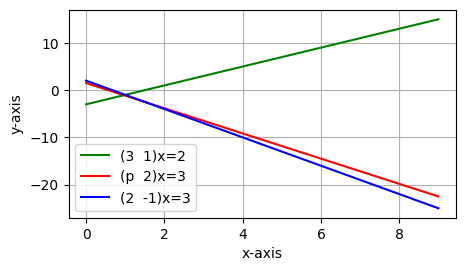
\includegraphics[width=\columnwidth]{fig/11.10.4.9.png}
    \caption{}
    \label{11.10.4.9}
\end{figure}
\end{document}

